\documentclass{article}

\usepackage[a4paper, left=1.5cm, right=1.5cm, top=2cm, bottom=2cm]{geometry}

\usepackage{../../../../components/components}

\usepackage{hyperref}
\usepackage{fancyhdr}
\usepackage{ccicons}
\usepackage{tikz}

% Configuration des en-têtes et pieds de page
\pagestyle{fancy}
\fancyhf{} % reset tout

\fancyhead[L]{Préparation CAPES}
\fancyhead[C]{Statistiques}
\fancyhead[R]{2026-2027}

\fancyfoot[L]{Ewen Rodrigues de Oliveira\\\ccbyncsa}
\fancyfoot[R]{\thepage}

\begin{document}

\docTitle{Chapitre 2 : Séries statistiques à deux variables}

\noindent Ce chapitre est dédié à l'étude conjointe de deux caractères quantitatifs mesurés sur une même population. L'objectif est d'analyser l'existence d'une éventuelle relation mathématique (notamment linéaire) entre ces deux variables afin de proposer des modèles prédictifs.\\

\section{Nuage de points et point moyen}

\definition{
    Soit $\Omega$ une population finie de cardinal $N \in \mathbb{N}^*$. 
    On appelle \textbf{série statistique à deux variables} la donnée d'un $N$-uplet de couples $\left((x_1, y_1), (x_2, y_2), \dots, (x_N, y_N)\right) \in (\mathbb{R}^2)^N$, où $x_i$ et $y_i$ désignent les mesures respectives de deux caractères quantitatifs $X$ et $Y$ sur le même individu $i$ de la population.
}

\definition{
    Dans un repère cartésien du plan, l'ensemble des points $M_i(x_i, y_i)$ pour $i \in \{1, \dots, N\}$ est appelé le \textbf{nuage de points} associé à la série statistique.
}

\definition{
    On appelle \textbf{point moyen} du nuage de points, noté $G$, le point dont les coordonnées $(\bar{x}, \bar{y})$ sont les moyennes respectives des séries marginales $X$ et $Y$ :
    \[ \bar{x} = \frac{1}{N} \sum_{i=1}^{N} x_i \quad \text{et} \quad \bar{y} = \frac{1}{N} \sum_{i=1}^{N} y_i \]
}

\theorem{Propriété}{}{false}{
    Le point moyen $G$ correspond à l'isobarycentre du système de points $\left\{(M_1, 1), (M_2, 1), \dots, (M_N, 1)\right\}$. Autrement dit, il vérifie la relation vectorielle :
    \[ \sum_{i=1}^{N} \overrightarrow{GM_i} = \vec{0} \]
}

\noindent{\textbf{Preuve :}\\
    Exprimons les coordonnées du vecteur $\sum_{i=1}^{N} \overrightarrow{GM_i}$ dans le repère du plan :
    \[ \sum_{i=1}^{N} (x_i - \bar{x}) = \sum_{i=1}^{N} x_i - \sum_{i=1}^{N} \bar{x} = N\bar{x} - N\bar{x} = 0 \]
    De même pour l'ordonnée :
    \[ \sum_{i=1}^{N} (y_i - \bar{y}) = \sum_{i=1}^{N} y_i - \sum_{i=1}^{N} \bar{y} = N\bar{y} - N\bar{y} = 0 \]
    Les coordonnées de la somme vectorielle étant nulles, on a bien $\sum_{i=1}^{N} \overrightarrow{GM_i} = \vec{0}$. \hfill $\square$
}
\example{
    Une entreprise de logistique étudie la relation entre la distance parcourue par ses livreurs (en centaines de kilomètres, notée $X$) et la consommation de carburant associée (en litres, notée $Y$). Les données collectées sur un échantillon de $N = 5$ trajets sont résumées dans le tableau suivant :
\begin{center}
    \renewcommand{\arraystretch}{1.5} % Augmente la hauteur des cases
    \begin{tabular}{|l|c|c|c|c|c|}
        \hline
        Trajet ($i$) & 1 & 2 & 3 & 4 & 5 \\
        \hline
        Distance $x_i$ (en centaines de km) & 1 & 2 & 3 & 4 & 5 \\
        \hline
        Consommation $y_i$ (en litres) & 5 & 8 & 11 & 11 & 15 \\
        \hline
    \end{tabular}
\end{center}

    \begin{enumerate}
        \item Calculons les moyennes respectives des variables marginales $X$ et $Y$ :
        \[ \bar{x} = \frac{1 + 2 + 3 + 4 + 5}{5} = \frac{15}{5} = 3 \]
        \[ \bar{y} = \frac{5 + 8 + 11 + 11 + 15}{5} = \frac{50}{5} = 10 \]
        Le point moyen du nuage a donc pour coordonnées \textbf{$G(3 ; 10)$}.
        
        \item \textbf{Représentation graphique (Nuage de points et point $G$) :}
    \end{enumerate}

    \begin{center}
        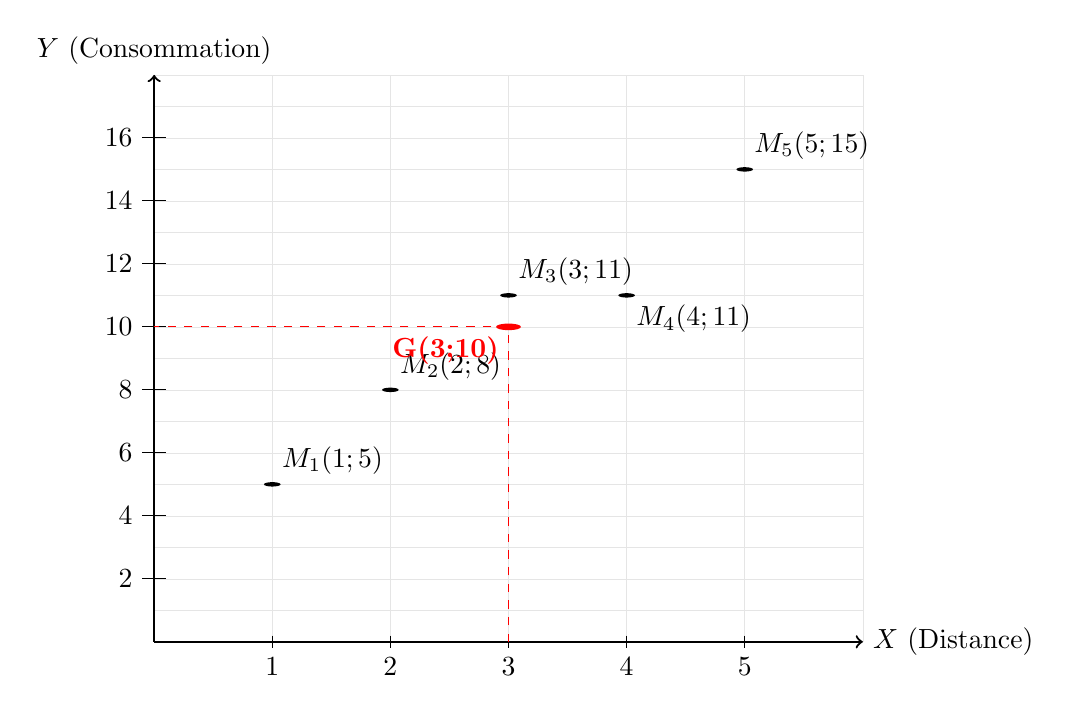
\begin{tikzpicture}[xscale=1.5, yscale=0.4]
            % Grille de fond
            \draw[gray!20, very thin, step=1] (0,0) grid (6,18);
            
            % Axes
            \draw[->, thick] (0,0) -- (6,0) node[right] {$X$ (Distance)};
            \draw[->, thick] (0,0) -- (0,18) node[above] {$Y$ (Consommation)};
            
            % Graduations axe X
            \foreach \x in {1,2,3,4,5}
                \draw (\x,0.2) -- (\x,-0.2) node[below] {\x};
                
            % Graduations axe Y
            \foreach \y in {2,4,6,8,10,12,14,16}
                \draw (0.1,\y) -- (-0.1,\y) node[left] {\y};
            
            % Points du nuage (M_i)
            \fill (1,5) circle (2pt) node[above right] {$M_1(1;5)$};
            \fill (2,8) circle (2pt) node[above right] {$M_2(2;8)$};
            \fill (3,11) circle (2pt) node[above right] {$M_3(3;11)$};
            \fill (4,11) circle (2pt) node[below right] {$M_4(4;11)$};
            \fill (5,15) circle (2pt) node[above right] {$M_5(5;15)$};
            
            % Point moyen G en rouge
            \fill[red] (3,10) circle (3pt) node[below left, red] {\textbf{G(3;10)}};
            \draw[red, dashed] (3,0) -- (3,10) -- (0,10);
        \end{tikzpicture}
    \end{center}
}

\section{Outils de liaison}

\subsection{La Covariance}

\definition{
    On appelle \textbf{covariance} des variables $X$ et $Y$, notée $\text{Cov}(X,Y)$ ou $\sigma_{XY}$, le réel défini par la moyenne des produits des écarts aux moyennes respectives :
    \[ \text{Cov}(X,Y) = \frac{1}{N} \sum_{i=1}^{N} (x_i - \bar{x})(y_i - \bar{y}) \]
}

\theorem{Théorème}{Formule de König-Huygens pour la covariance}{false}{
    La covariance est égale à la moyenne des produits des valeurs moins le produit de leurs moyennes :
    \[ \text{Cov}(X,Y) = \left( \frac{1}{N} \sum_{i=1}^{N} x_i y_i \right) - \bar{x}\bar{y} \]
}

\noindent{\textbf{Preuve :}\\
    Développons le terme sous la somme de la définition :
    \[ \text{Cov}(X,Y) = \frac{1}{N} \sum_{i=1}^{N} (x_i y_i - x_i \bar{y} - \bar{x} y_i + \bar{x}\bar{y}) \]
    Par linéarité de la sommation et en sortant les constantes $\bar{x}$ et $\bar{y}$ de chaque somme partielle :
    \[ \text{Cov}(X,Y) = \frac{1}{N} \sum_{i=1}^{N} x_i y_i - \bar{y} \left(\frac{1}{N} \sum_{i=1}^{N} x_i\right) - \bar{x} \left(\frac{1}{N} \sum_{i=1}^{N} y_i\right) + \frac{1}{N} \sum_{i=1}^{N} \bar{x}\bar{y} \]
    Comme $\frac{1}{N}\sum x_i = \bar{x}$, $\frac{1}{N}\sum y_i = \bar{y}$ et $\frac{1}{N}\sum \bar{x}\bar{y} = \bar{x}\bar{y}$, on obtient :
    \[ \text{Cov}(X,Y) = \left(\frac{1}{N} \sum_{i=1}^{N} x_i y_i\right) - \bar{y}(\bar{x}) - \bar{x}(\bar{y}) + \bar{x}\bar{y} \]
    \[ \text{Cov}(X,Y) = \left(\frac{1}{N} \sum_{i=1}^{N} x_i y_i\right) - \bar{x}\bar{y} \hfill \square \]
}

\example{
    Un chercheur en écologie souhaite étudier la relation entre la taille d'une plante (en cm, notée $X$) et le nombre de fleurs qu'elle produit (noté $Y$). Les données collectées sur un échantillon de $N = 6$ plantes sont les suivantes :
\begin{center}
    \renewcommand{\arraystretch}{1.5} % Augmente la hauteur des cases
    \begin{tabular}{|l|c|c|c|c|c|c|}
        \hline
        Plante ($i$) & 1 & 2 & 3 & 4 & 5 & 6 \\
        \hline
        Taille $x_i$ (en cm) & 10 & 15 & 20 & 25 & 30 & 35 \\
        \hline
        Nombre de fleurs $y_i$ & 2 & 3 & 5 & 7 & 11 & 13 \\
        \hline
    \end{tabular}
\end{center}

On veut calculer la covariance entre les variables $X$ et $Y$ pour évaluer la force de leur relation linéaire à l'aide de deux méthodes (à partir de la définition, puis à partir de la formule de König-Huygens).\\
Calculons les moyennes respectives des variables marginales $X$ et $Y$ sous forme fractionnaire simplifiée :
\[ \bar{x} = \frac{10 + 15 + 20 + 25 + 30 + 35}{6} = \frac{135}{6} = \frac{45}{2} \]
\[ \bar{y} = \frac{2 + 3 + 5 + 7 + 11 + 13}{6} = \frac{41}{6} \]

\begin{enumerate}
    \item \textbf{Calcul à partir de la définition de la covariance :}
    \[ \text{Cov}(X,Y) = \frac{1}{6} \sum_{i=1}^{6} (x_i - \bar{x})(y_i - \bar{y}) \]
    Calculons les produits des écarts sous forme de fractions pour chaque plante :
    \begin{align*}
        \left(10 - \frac{45}{2}\right)\left(2 - \frac{41}{6}\right) &= \left(-\frac{25}{2}\right)\left(-\frac{29}{6}\right) = \frac{725}{12} \\
        \left(15 - \frac{45}{2}\right)\left(3 - \frac{41}{6}\right) &= \left(-\frac{15}{2}\right)\left(-\frac{23}{6}\right) = \frac{345}{12} \\
        \left(20 - \frac{45}{2}\right)\left(5 - \frac{41}{6}\right) &= \left(-\frac{5}{2}\right)\left(-\frac{11}{6}\right) = \frac{55}{12} \\
        \left(25 - \frac{45}{2}\right)\left(7 - \frac{41}{6}\right) &= \left(\frac{5}{2}\right)\left(\frac{1}{6}\right) = \frac{5}{12} \\
        \left(30 - \frac{45}{2}\right)\left(11 - \frac{41}{6}\right) &= \left(\frac{15}{2}\right)\left(\frac{25}{6}\right) = \frac{375}{12} \\
        \left(35 - \frac{45}{2}\right)\left(13 - \frac{41}{6}\right) &= \left(\frac{25}{2}\right)\left(\frac{37}{6}\right) = \frac{925}{12}
    \end{align*}
    En sommant ces produits, on obtient :
    \[ \sum_{i=1}^{6} (x_i - \bar{x})(y_i - \bar{y}) = \frac{725 + 345 + 55 + 5 + 375 + 925}{12} = \frac{2430}{12} = \frac{405}{2} \]
    Ainsi, la covariance est :
    \[ \text{Cov}(X,Y) = \frac{1}{6} \times \frac{405}{2} = \frac{405}{12} = \frac{135}{4} \]

    \item \textbf{Calcul à partir de la formule de König-Huygens :}
    La formule de König-Huygens pour la covariance est donnée par :
    \[ \text{Cov}(X,Y) = \left( \frac{1}{6} \sum_{i=1}^{6} x_i y_i \right) - \bar{x}\bar{y} \]
    Calculons la somme des produits $x_i y_i$ :
    \begin{align*}
        \sum_{i=1}^{6} x_i y_i &= (10 \times 2) + (15 \times 3) + (20 \times 5) + (25 \times 7) + (30 \times 11) + (35 \times 13) \\
        &= 20 + 45 + 100 + 175 + 330 + 455 = 1125
    \end{align*}
    La moyenne de ces produits vaut :
    \[ \frac{1}{6} \sum_{i=1}^{6} x_i y_i = \frac{1125}{6} = \frac{375}{2} \]
    Par soustraction du produit des deux moyennes marginales, on obtient :
    \[ \text{Cov}(X,Y) = \frac{375}{2} - \left(\frac{45}{2} \times \frac{41}{6}\right) = \frac{375}{2} - \frac{1845}{12} = \frac{2250 - 1845}{12} = \frac{405}{12} = \frac{135}{4} \]
\end{enumerate}

Les deux méthodes aboutissent exactement au même résultat rationnel de $\frac{135}{4}$. La covariance positive indique que la taille de la plante et son nombre de fleurs évoluent de manière globalement croissante. \hfill $\square$
}

\subsection{Coefficient de corrélation linéaire}

\definition{
    On appelle \textbf{coefficient de corrélation linéaire} de Bravais-Pearson entre $X$ et $Y$, noté $r(X,Y)$, le réel défini par :
    \[ r(X,Y) = \frac{\text{Cov}(X,Y)}{\sigma_X \sigma_Y} \]
    où $\sigma_X$ et $\sigma_Y$ sont les écarts-types non nuls respectifs des séries marginales $X$ et $Y$.
}

\theorem{Théorème}{Bornes du coefficient de corrélation}{false}{
    Pour toute série statistique à deux variables, le coefficient de corrélation linéaire vérifie :
    \[ -1 \le r(X,Y) \le 1 \quad (\text{soit } |r(X,Y)| \le 1) \]
}

\noindent{\textbf{Preuve (via l'inégalité de Cauchy-Schwarz) :}\\
    Considérons l'espace vectoriel numérique $\mathbb{R}^N$ muni de son produit scalaire usuel $\langle u, v \rangle = \sum_{i=1}^N u_i v_i$. L'inégalité de Cauchy-Schwarz affirme que $\langle u, v \rangle^2 \le \|u\|^2 \|v\|^2$.\\
    Posons, pour chaque $i \in \{1, \dots, N\}$, les composantes des vecteurs $u$ et $v$ :
    \[ u_i = (x_i - \bar{x})\sqrt{\frac{1}{N}} \quad \text{et} \quad v_i = (y_i - \bar{y})\sqrt{\frac{1}{N}} \]
    Calculons la norme au carré de $u$ et $v$ :
    \[ \|u\|^2 = \sum_{i=1}^N u_i^2 = \frac{1}{N}\sum_{i=1}^N (x_i - \bar{x})^2 = V(X) = \sigma_X^2 \]
    \[ \|v\|^2 = \sum_{i=1}^N v_i^2 = \frac{1}{N}\sum_{i=1}^N (y_i - \bar{y})^2 = V(Y) = \sigma_Y^2 \]
    Calculons le produit scalaire $\langle u, v \rangle$ :
    \[ \langle u, v \rangle = \sum_{i=1}^N u_i v_i = \frac{1}{N}\sum_{i=1}^N (x_i - \bar{x})(y_i - \bar{y}) = \text{Cov}(X,Y) \]
    L'inégalité de Cauchy-Schwarz s'écrit alors :
    \[ \left(\text{Cov}(X,Y)\right)^2 \le \sigma_X^2 \cdot \sigma_Y^2 \]
    Puisque $\sigma_X > 0$ et $\sigma_Y > 0$, en prenant la racine carrée, on obtient :
    \[ |\text{Cov}(X,Y)| \le \sigma_X \sigma_Y \implies \frac{|\text{Cov}(X,Y)|}{\sigma_X \sigma_Y} \le 1 \implies |r(X,Y)| \le 1 \hfill \square \]
}

\section{Ajustement affine par la méthode des moindres carrés}

Lorsque le nuage de points présente une forme allongée, on cherche à modéliser la relation entre $Y$ et $X$ par une fonction affine $y = ax + b$.

\definition{
    La \textbf{droite de régression de $Y$ en $X$} par la méthode des moindres carrés est la droite d'équation $y = ax + b$ qui minimise la somme des carrés des écarts verticaux entre les points du nuage et la droite. Elle minimise la fonction :
    \[ f(a,b) = \sum_{i=1}^{N} (y_i - (ax_i + b))^2 \]
}

\theorem{Théorème}{Détermination des coefficients $a$ et $b$}{false}{
    La fonction $f(a,b)$ admet un minimum global unique pour les coefficients définis par :
    \[ a = \frac{\text{Cov}(X,Y)}{V(X)} \quad \text{et} \quad b = \bar{y} - a\bar{x} \]
}

\noindent{\textbf{Preuve (par l'annulation du gradient) :}\\
    La fonction $f$ est une fonction de deux variables $a$ et $b$, strictement convexe, de classe $\mathcal{C}^{\infty}$ sur $\mathbb{R}^2$. Son minimum unique est donné par l'annulation de ses dérivées partielles.\\
    Calculons la dérivée partielle de $f$ par rapport à $b$ :
    \[ \frac{\partial f}{\partial b}(a,b) = -2 \sum_{i=1}^{N} (y_i - ax_i - b) = 0 \implies \sum_{i=1}^{N} y_i - a\sum_{i=1}^{N} x_i - \sum_{i=1}^{N} b = 0 \]
    En divisant par $N$, on obtient immédiatement la relation :
    \[ \bar{y} - a\bar{x} - b = 0 \implies b = \bar{y} - a\bar{x} \quad \text{(1)} \]
    Calculons maintenant la dérivée partielle de $f$ par rapport à $a$ :
    \[ \frac{\partial f}{\partial a}(a,b) = -2 \sum_{i=1}^{N} x_i(y_i - ax_i - b) = 0 \implies \sum_{i=1}^{N} x_i y_i - a\sum_{i=1}^{N} x_i^2 - b\sum_{i=1}^{N} x_i = 0 \]
    Injectons la relation (1) pour éliminer la variable $b$ :
    \[ \sum_{i=1}^{N} x_i y_i - a\sum_{i=1}^{N} x_i^2 - (\bar{y} - a\bar{x})\sum_{i=1}^{N} x_i = 0 \]
    En divisant le tout par $N$ :
    \[ \left(\frac{1}{N}\sum_{i=1}^{N} x_i y_i\right) - a\left(\frac{1}{N}\sum_{i=1}^{N} x_i^2\right) - \bar{y}\bar{x} + a\bar{x}^2 = 0 \]
    Regroupons les termes en $a$ :
    \[ \left[\left(\frac{1}{N}\sum_{i=1}^{N} x_i y_i\right) - \bar{x}\bar{y}\right] - a \left[\left(\frac{1}{N}\sum_{i=1}^{N} x_i^2\right) - \bar{x}^2\right] = 0 \]
    On reconnaît les formules de König-Huygens pour la covariance et la variance de $X$ :
    \[ \text{Cov}(X,Y) - a V(X) = 0 \implies a = \frac{\text{Cov}(X,Y)}{V(X)} \hfill \square \]
}

\remark{
    Puisque $b = \bar{y} - a\bar{x}$, l'équation de la droite peut s'écrire sous la forme $y - \bar{y} = a(x - \bar{x})$. Ceci démontre géométriquement que la droite de régression passe impérativement par le \textbf{point moyen $G(\bar{x}, \bar{y})$}.
}

\example{
    Reprenons l'exemple de l'entreprise de logistique avec les données suivantes :
\begin{center}
    \renewcommand{\arraystretch}{1.5} % Augmente la hauteur des cases
    \begin{tabular}{|l|c|c|c|c|c|}
        \hline
        Trajet ($i$) & 1 & 2 & 3 & 4 & 5 \\
        \hline
        Distance $x_i$ (en centaines de km) & 1 & 2 & 3 & 4 & 5 \\
        \hline
        Consommation $y_i$ (en litres) & 5 & 8 & 11 & 11 & 15 \\
        \hline
    \end{tabular}
\end{center}

Déterminons l'équation de la droite de régression de $Y$ en $X$ sous forme fractionnaire :
\begin{itemize}
    \item \textbf{Calcul de la covariance $\text{Cov}(X,Y)$ :}
    On rappelle que $\bar{x} = 3$ et $\bar{y} = 10$.
    \[ \text{Cov}(X,Y) = \frac{1}{5} \sum_{i=1}^{5} (x_i - \bar{x})(y_i - \bar{y}) \]
    \[ \text{Cov}(X,Y) = \frac{1}{5} \left[ (1-3)(5-10) + (2-3)(8-10) + (3-3)(11-10) + (4-3)(11-10) + (5-3)(15-10) \right] \]
    \[ \text{Cov}(X,Y) = \frac{1}{5} \left[ (-2)(-5) + (-1)(-2) + (0)(1) + (1)(1) + (2)(5) \right] \]
    \[ \text{Cov}(X,Y) = \frac{1}{5} (10 + 2 + 0 + 1 + 10) = \frac{23}{5} \]
    
    \item \textbf{Calcul de la variance $V(X)$ :}
    \[ V(X) = \frac{1}{5} \sum_{i=1}^{5} (x_i - \bar{x})^2 \]
    \[ V(X) = \frac{1}{5} \left[ (1-3)^2 + (2-3)^2 + (3-3)^2 + (4-3)^2 + (5-3)^2 \right] \]
    \[ V(X) = \frac{1}{5} (4 + 1 + 0 + 1 + 4) = \frac{10}{5} = 2 \]
    
    \item \textbf{Calcul des coefficients $a$ et $b$ :}
    \[ a = \frac{\text{Cov}(X,Y)}{V(X)} = \frac{\frac{23}{5}}{2} = \frac{23}{10} \]
    \[ b = \bar{y} - a\bar{x} = 10 - \frac{23}{10} \times 3 = 10 - \frac{69}{10} = \frac{100 - 69}{10} = \frac{31}{10} \]
\end{itemize}

L'équation de la droite de régression de $Y$ en $X$ par la méthode des moindres carrés est donc :
\[ y = \frac{23}{10}x + \frac{31}{10} \]
}

\section{Applications prédictives : Interpolation et extrapolation}

Une fois le modèle linéaire $y = ax + b$ validé par un coefficient de corrélation proche de $1$ ou de $-1$, il devient possible d'estimer des valeurs inconnues.

\definition{
    Soit $x_{\text{estim}}$ une valeur pour laquelle on souhaite évaluer la valeur de $y$ correspondante à l'aide de l'équation de la droite d'ajustement.
    \begin{itemize}
        \item On parle d'\textbf{interpolation} si la valeur $x_{\text{estim}}$ se situe à l'intérieur de l'intervalle des données observées de la série : $x_{\text{estim}} \in [x_1 ; x_k]$. Ce procédé est généralement considéré comme fiable si le coefficient de corrélation est fort.
        \item On parle d'\textbf{extrapolation} si la valeur $x_{\text{estim}}$ se situe en dehors de l'intervalle des valeurs observées : $x_{\text{estim}} < x_1$ ou $x_{\text{estim}} > x_k$. Ce procédé est plus risqué car il suppose que le comportement linéaire constaté reste valable en dehors du cadre de l'étude.
    \end{itemize}
}
\example{
    Reprenons la droite d'ajustement affine obtenue pour l'entreprise de logistique, dont l'équation est :
    \[ y = \frac{23}{10}x + \frac{31}{10} \quad (\text{soit } y = 2,3x + 3,1) \]
    On rappelle que les distances observées dans l'échantillon initial s'étendent de $x_1 = 1$ à $x_5 = 5$ (en centaines de kilomètres).

    \begin{enumerate}
        \item \textbf{Cas d'une interpolation :}\\
        L'entreprise souhaite estimer la consommation de carburant pour un trajet prévu de $250$ km, soit $x_{\text{estim}} = 2,5$. \\
        Puisque $2,5 \in [1 ; 5]$, il s'agit d'une \textbf{interpolation}. En utilisant le modèle, on obtient :
        \[ y = 2,3 \times 2,5 + 3,1 = 5,75 + 3,1 = 8,85 \text{ litres} \]
        Cette estimation est considérée comme hautement fiable car elle s'effectue au sein du domaine d'observation où le comportement linéaire a été formellement validé.

        \item \textbf{Cas d'une extrapolation :}\\
        L'entreprise souhaite désormais évaluer la consommation pour un long trajet de $1200$ km, soit $x_{\text{estim}} = 12$. \\
        Puisque $12 > 5$, il s'agit d'une \textbf{extrapolation}. Le modèle donne :
        \[ y = 2,3 \times 12 + 3,1 = 27,6 + 3,1 = 30,7 \text{ litres} \]
        Cette estimation est sujette à caution. En effet, rien ne garantit que la consommation du véhicule reste strictement linéaire sur une distance aussi grande (des facteurs comme la fatigue du moteur, le type de routes empruntées ou la capacité du réservoir pourraient modifier le comportement du caractère en dehors de l'intervalle $[1 ; 5]$).
    \end{enumerate}
}

\newpage
\tableofcontents

\section*{Crédits}
Ce cours est mis à disposition selon les termes de la Licence Creative Commons \ccbyncsa\ \textbf{Attribution - Pas d'Utilisation Commerciale - Partage dans les Mêmes Conditions 4.0 International}. 
Pour voir une copie de cette licence, visitez \url{http://creativecommons.org/licenses/by-nc-sa/4.0/}.

\end{document}